\documentclass{notes}


\begin{document}

\section{Introduction}

Rod 的定义是 $L \gg r$ 的柱体,也就是常说的细绳、细杆。

因此,虽然万物皆可有限元(因为万物皆有广延),但是我们为了模型的简化,依然把 Rod 看作是一维的物体对其进行一维的建模。但除此之外,Rod 的模拟和我之前做的有限元模拟,没有什么大的套路上的区别。

在这篇文章中,我们只研究不可拉伸的 rod,因此所有研究的 rod 都是可以弧长参数化的。

\section{Math Preliminary}

\subsection{Connection and Darboux Vector}

微分几何中,标架场 $\left\lbrace x; e_i \right\rbrace$ 的联络(connection)$\omega^i, \omega^j_i$ 被定义如下:

\begin{equation}
	\begin{aligned}
		&dx = \omega^i e_i \\
		&de_i = \omega_i^j e_j
	\end{aligned}
\end{equation}

并且我们有:

\begin{equation}
	\omega_i^j = - \omega_j^i
\end{equation}

(证明留作习题)

在这里,$\omega^i$ 和 $\omega^j_i$ 都是一阶外微分。如果标架场是一维的,那么外微分均可以表示成 $a\ ds, a \in \mathbb{R}$ 的形式,因此,我们可以直接用一组系数来表示联络。下文中涉及到的标架场均是一维的,所以我们直接用 $\omega$ 来表示这组系数,而不会产生歧义。即标架场 $\left\lbrace x(s); e_i(s) \right\rbrace$ 的联络系数为:

\begin{equation}
	\begin{aligned}
		&\dot{x} = \omega^i e_i \\
		&\dot{e}_i = \omega_i^j e_j
	\end{aligned}
\end{equation}

我刚学微分几何的时候,觉得这个公式也就是形式上的意义,直到接触了这篇文章,我才意识到原来联络系数是有几何意义的,注意到:

$$
	\begin{aligned}
		\dot{e}_1 &= \omega_1^2 e_2 + \omega_1^3 e_3 \\
		&= \omega_1^2 e_3 \times e_1 + \omega_3^1 e_2 \times e_1 \\
		&= (\omega_1^2 e_3 + \omega_3^1 e_2) \times e_1
	\end{aligned}
$$

所以,实际上 $\omega_1^2$ 和 $\omega_3^1$ 分别表征了 \textbf{$e_1$ 绕着 $e_3, e_2$ 轴旋转的角速度}。

类似的公式对 $e_2, e_3$ 自然也成立,最终我们得到:

\begin{equation}\label{eq:darboux}
	\begin{aligned}
		\omega &= \omega_2^3 e_1 + \omega_3^1 e_2 + \omega_1^2 e_3 \\
		&\Rightarrow \dot{e}_i = \omega \times e_i
	\end{aligned}
\end{equation}

我们把 $\omega$ 称为 Darboux 向量。

\subsection{Bishop Frame}

曲线上的标架场有无穷多种,即使固定其中一个标架为单位切向量也一样。我们最熟悉的标架场为 Frenet 标架场 $\left\lbrace x; T, N, B \right\rbrace$。Frenet 标架的优点在于其联络系数具有几何意义,而且三个独立的联络系数之中只有两个非零。但它仍然有一大缺点:在非孤立的 $\ddot{x} = 0$ 的点(二阶奇点)处无法定义(在孤立的二阶奇点处可以根据连续性定义),也就是如果曲线中间有一段是直的,Frenet 标架就无法定义了,这是我们无法接受的。我们接下来介绍的 Bishop 标架在继承了 Frenet 标架的优点的同时,避免了 Frenet 标架的缺点。

\begin{definition}
	若曲线 $C$ 的法向量场 $M$ 满足 $M' \parallel T$,其中 $T$ 为 $C$ 的切向量场则称 $M$ 为相对平行(relatively parallel)的,称 $M$ 为相对平行法向量场(relatively parallel normal vector field,RPNVF)
\end{definition}

\begin{remark}
	在英文中要注意区分一下 normal vector 的含义,有时候它指的是主法向量,有时候它指的是任意垂直于切向量的向量,这里取第二种意思。

	以下若不加特殊说明,切向量均默认长度为 $1$
\end{remark}

容易验证,若 $M$ 是相对平行法向量场,$T \times M$ 也是相对平行法向量场,三者组成一个标架(当然,需要 normalize 一下)。

显然,如果曲线的法向量绕着切向量旋转,其结果将仍然是法向量。而 $M' = c_0T = c_1 (M \times T) \times M$ 则说明了 $M$ 没有围绕 $T$ 旋转。\textbf{它仅仅为了保持自己和切向量垂直作了旋转,因此它的旋转是所有法向量场中“最小”的},这是相对平行法向量场的特点。

RPNVF 有如下性质:

\begin{proposition}
	RPNVF 的向量长度相同。
\end{proposition}

\begin{proof}
	由于 $M' \parallel T$,故 $M' \cdot M = 0 \Rightarrow (M \cdot M)' = 0 \Rightarrow || M || = const.$
\end{proof}

至此,我们可能会对为什么这样的向量场叫做“相对平行”感到奇怪,它得名于如下的性质

\begin{proposition}
	$x: [0, l] \rightarrow \mathbb{R}^3$ 为一光滑曲线,$M$ 是它的 RPNVF,则曲线 $\tilde{x} = x + M$ 满足 $M$ 同时是 $x$ 和 $\tilde{x}$ 的法向量,此时由于 $M$ 定长,二者距离保持不变——即二者“平行”。
\end{proposition}

\begin{proof}
	设 $s$ 为 $x$ 的弧长参数,以及 $\frac{dM}{ds} = cT$,则:
	$\frac{d\tilde{x}}{d\tilde{s}} = \frac{d \tilde{x}}{d s} \frac{ds}{d \tilde{s}} = (T + cT) \frac{ds}{d\tilde{s}} \perp M$
	而 $M$ 又是 $x$ 的法向量场,所以 $M$ 同时垂直于两曲线。
\end{proof}

\begin{remark}
	是不是有点像 Bertrand 曲线?不过 Bertrand 曲线要求主法向量相同,这里只要求法向量相同。
\end{remark}

至此,我们已经知道了 RPNVF 的不少有用性质,但是还不知道 RPNVF 是否存在。

\begin{theorem}
	对任意光滑曲线 $x: [0, l] \rightarrow \mathbb{R}^3$,其 RPNVF 均存在,且若给定初始值 $M(0) = M_0 \perp T(0)$,则这样的 RPNVF 是唯一的
\end{theorem}

\begin{proof}
	先证明唯一性,显然,若 $M_1, M_2$ 都是 RPNVF,则根据定义 $M_1 - M_2$ 也是 RPNVF,若 $M_1, M_2$ 具有相同的初始值,则 $(M_1 - M_2)(0) = 0$,而 RPNVF 定长,故 $M_1 \equiv M_2$

	再证明存在性,由于等比缩放一个 RPNVF 后仍然是 RPNVF,所以我们等价的要找到一个单位长的 RPNVF。为此,我们首先取标架 $\left\lbrace T, N_1, N_2 \right\rbrace$,其中 $N_1, N_2$ 由 $T$ 直接 Graham-Schimidt 分解得来的单位向量。此时 $M$ 一定可以表示成 $\cos(\theta) N_1(s) + \sin (\theta) N_2(s)$ 的形式,其中 $\theta$ 为 $s$ 的函数。求导,利用联络系数得到:

	$$
		\begin{aligned}
		M' &= - \sin (\theta) \theta' N_1 + \cos (\theta) \theta' N_2 + \cos(\theta) (\omega_{2}^1 T + \omega_2^3 N_2) + \sin(\theta) (\omega_3^1 T + \omega_3^2 N_1) \\
		&= - \sin \theta(\theta' - \omega_3^2) N_1 + \cos \theta(\theta' - \omega_3^2) N_2 + (\cos \theta \omega_2^1 + \sin \theta \omega_3^1)T
		\end{aligned}
	$$

	可见,要使得 $M' \parallel T$,当且仅当 $\theta' = \omega_3^2$ 恒成立。而 $\omega_3^2$ 连续,故常微分方程在 $[0, l]$ 上有解,即存在 RPNVF。
\end{proof}

\begin{definition}
	若曲线 $C$ 的切向量场 $M$ 定长,则称之为 $C$ 的相对平行切向量场 
\end{definition}

\begin{definition}
	若曲线 $C$ 上的向量场的切向分量和法向分量都相对平行,则称其为 $C$ 的相对平行向量场,或者简称相对平行场
\end{definition}

相对平行法向量场的存在唯一性基础上我们能够很快得出相对平行场的存在唯一性。

\begin{theorem}
	对任意光滑曲线 $x: [0, l] \rightarrow \mathbb{R}^3 \in \mathcal{C}^k$,其相对平行向量场 $V \in \mathcal{C}^{k - 1}$ 均存在,且若给定初始值 $V(0) = V_0$,则这样的相对平行向量场是唯一的。并且任意两个相对平行场的内积是固定的。
\end{theorem}

\begin{proof}
	存在唯一性证明略。至于内积固定,只需要注意到 $<U, V>' = <c_1T, V> + <U, c_2T> = 0$
\end{proof}

上面的定理是很不平凡的,最关键的是,它说明了相对平行场可以由初始值完全确定(不过这也没啥好奇怪的,微分方程的解也是由初值完全确定的)。另外,注意到如果 $U, V$ 是相对平行场,则 $aU + bV$ 也是,而由于 $aU + bV$ 的初始值为 $aU_0 + bV_0$,再根据唯一性,初值为 $aU_0 + bV_0$ 的相对平行场一定是 $aU + bV$。因此,\textbf{相对平行场的集合是一个欧式空间 $\mathcal{U}$,且这个欧式空间和 $\mathbb{R}^3$ 同构,同构映射为 $U \rightarrow U_0$}

而根据我们刚才的讨论,这个线性空间可以拆分成两个正交补空间:(一维的)相对平行切向量空间 $\mathcal{T}$ 和(二维的)相对平行法向量空间 $\mathcal{N}$。我们在这两个空间中分别取正交基,构成 $\mathcal{U}$ 的一个正交基:

\begin{definition}
	对于光滑曲线 $C$,称由 $\mathcal{T}$ 和 $\mathcal{N}$ 的正交基构成的 $\mathcal{U}$ 的正交基为 $C$ 的相对平行标架场(relatively parallel adapted frame (field), RPAF)
\end{definition}

\begin{remark}
	这里 adapted 的意思是正交基中的一个向量为切向量,一般我们说 adapted frame 指的就是满足这一性质的标架。

	此外,在这里我们默认的所有标架场都是右手系。
\end{remark}

回到我们的问题上来,对于 RPAF $\left\lbrace T, M_1, M_2 \right\rbrace$ 由于 $\dot{M}_1, \dot{M}_2 \parallel T$,其联络系数满足下面的条件:

\begin{equation}
	\begin{aligned}
		\dot{T} &= & &-c_1 M_1 + &-c_2 M_2 \\
		\dot{M}_1 &= &c_1 T \\
		\dot{M}_2 &= &c_2 T
	\end{aligned}
\end{equation}

它的三个独立的联络系数也只有两个非零。

而且还有一点,RPAF 是除了 Frenet 标架之外唯一可能的只有两个非零的联络系数的标架。因为可能的情况无非是 $\omega_2^3 = 0$(RPAF),$\omega_1^3 = 0$(Frenet)和 $\omega_1^2 = 0$(也是 Frenet,但 $N, B$ 的位置互换)

由于 RPAF 是数学家 Bishop 提出的,我们一般称之为 Bishop frame。

\subsubsection{A discussion about the integrety of Bishop frame}

从上面的讨论可以看出 Bishop Frame 和 Frenet Frame 有一个本质区别。Bishop Frame 是一个\textbf{整体}的概念,任意给定一个曲线上的点,我们不能说出此处的 Bishop Frame 是什么,只有给定初值才能确定。

而 Frenet Frame 则是一个局部的概念,给定一个曲线的局部信息,我就可以完全确认出 Frenet Frame 来。

现在让我们考虑光滑的闭曲线 $x: S^1 \rightarrow \mathbb{R}^3$,因为 Frenet Frame 是局部的性质,所以标架 $\left\lbrace x; T, B, N \right\rbrace$ 是确定的单值函数。但 Bishop Frame 却可能是多值函数——因为当我固定 $M_1(0)$ 时,求解出来的 Bishop Frame 很可能会有 $M_1(2 \pi) \ne M_1(0)$。类似的事情在我们试图把 $\log$ 延陀到 $\mathbb{C}$ 上时就发生过。这一特性我们将在下文“平移”这一节中详细叙述。

\subsection{Parallel Transport, Connection and Holonomy}

在欧氏空间中,我们对“平移”这个概念并不陌生,若在点 $x$ 处有向量 $v$(二者合起来表示了一条有向线段),则将此向量从 $x$ 处平移到 $x + \Delta x$ 处后依然是 $v$——平移不会改变向量的坐标表示。

但对于一般的流形来说,“平移”就不是那么显然了。我们只有先定义流形上的“坐标系”,才能够把不同位置的坐标等同起来,认为他们是平移的结果。然而坐标系的定义是有讲究的,比方说之前选取的 Bishop 标架在定义平移的时候就会产生麻烦——同一个向量,“平移”一圈回来之后,竟会发现实际方向发生了变化。

\subsection{Writhe, Linking number and Twist}



\section{Physics Model}

\subsection{Material Frame and Elastic Energy}

尽管我们用一维的方式建模,但 rod 的物理实体还是三维的,所以它的物理属性,仍然是在三维上表述的。

我们假想 rod 是一根圆柱,圆柱的中心称为中轴线(centerline)。仅仅一根中轴线并不足以描述整个圆柱,因为在固定中轴线的时候,我们仍然可以在圆柱的横截面上对圆柱进行扭曲。物理上,为了刻画 rod 的扭转,我们为 rod 的中轴线赋予一个右手标架场 $\left\lbrace x; T, M_1, M_2 \right\rbrace$ ,称为材料标架(material frame)。其中 $T = \frac{dx}{ds}$ 为中轴线的切向量。材料标架是 rod 的物理属性而非数学属性。

简单来说,中轴线 $x$ 表示了 rod 的弯曲,而标架 $\left\lbrace T, M_1, M_2 \right\rbrace$ 则表征了 rod 的扭转。

\begin{figure}[H]
	\centering
	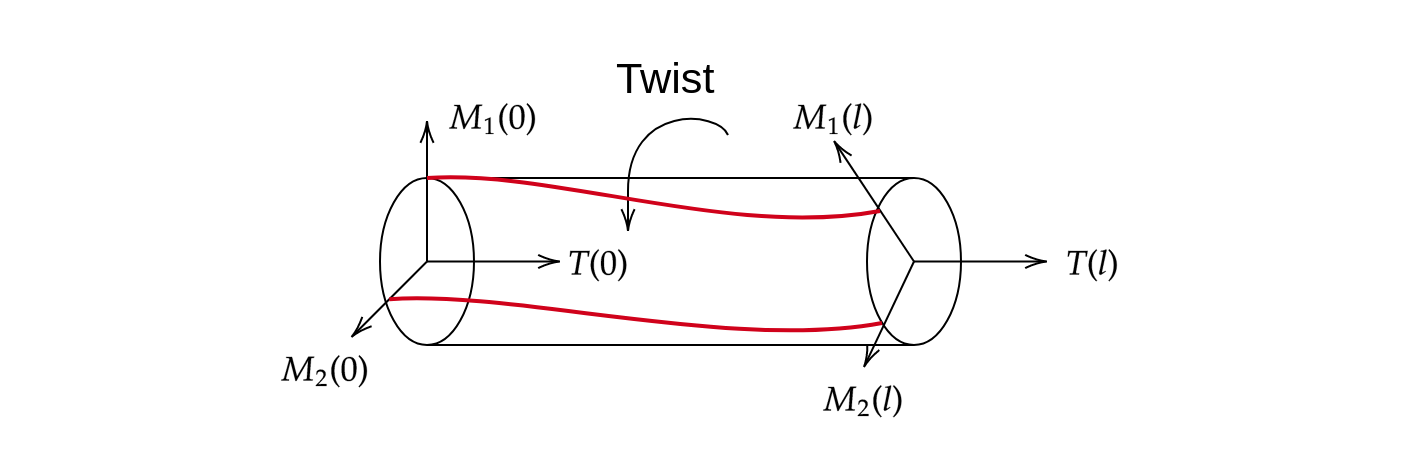
\includegraphics[width=0.85\textwidth]{img/Twist.png}
	\caption{Twist represented by material frame}
\end{figure}

对应的,rod 的能量也由这两项构成:

\begin{definition}
	对于由标架 $\left\lbrace x; T, M_1, M_2 \right\rbrace$ 表示的 rod $\Gamma$,由于其物理意义,我们特别将其联络系数记为 $\omega_1, \omega_2, m$:

	\begin{equation}
		\begin{aligned}
			\omega_1 &= \dot{T} \cdot M_1 \\
			\omega_2 &= \dot{T} \cdot M_2 \\
			m &= \dot{M}_1 \cdot M_2
		\end{aligned}
	\end{equation}
	
	且记 $\omega = \begin{bmatrix}\omega_1 \\ \omega_2\end{bmatrix}$

	则对于各项同性、rest shape 为直线的 rod,其能量表达式如下:
	\begin{equation}
		\begin{aligned}
			E(\Gamma) &= E_{bend}(\Gamma) + E_{twist}(\Gamma) \\
			E_{bend} &= \frac{1}{2} \int_{0}^{l} \alpha \omega^2 ds \\
			E_{twist} &= \frac{1}{2} \int_{0}^{l} \beta m^2 ds
		\end{aligned}
	\end{equation}
\end{definition}

\begin{remark}
	根据 \ref{eq:darboux},$m$ 的物理含义为 $M_1$ 绕 $T$ 轴旋转的角速度,称为 rod 的扭转(twist)。而 $\omega^2 = \omega \cdot \omega = || \dot{T} ||^2 = k^2$ 为曲率的平方。因此 $E_{bend}$ 惩罚了中轴线的弯曲,而 $E_{twist}$ 惩罚了材料标架围绕中轴线的旋转。
\end{remark}

对于非各项同性,rest shape 非直线的 rod,其能量表达式可以泛化成下面的形式:

\begin{definition}
	对于各项异性、rest shape 为任意形状的 rod,其能量表达式如下:

	\begin{equation}
		\begin{aligned}
			E(\Gamma) &= E_{bend}(\Gamma) + E_{twist}(\Gamma) \\
			E_{bend} &= \frac{1}{2} \int_{0}^{l} (\omega - \bar{\omega})^T B (\omega - \bar{\omega}) ds \\
			E_{twist} &= \frac{1}{2} \int_{0}^{l} \beta m^2 ds
		\end{aligned}
	\end{equation}

	其中 $B \in SPD(2)$ 由 rod 的物理性质决定。$\bar{\omega} = \omega_{rest\ shape}$ 
\end{definition}

\begin{remark}
	各项同性是 $B = \alpha I_2$ 的特例,rest shape 为直线是 $\bar{\omega} = 0$ 的特例
\end{remark}

以后若不加说明,我们均假设各向异性、rest shape 非直线。

\subsection{Introduction of Bishop Frame}

使用 $\left\lbrace x; T, M_1, M_2 \right\rbrace$ 来表示 rod 是有点浪费的。因为 $T = \dot{x}$ 完全由 $x$ 决定,如果我们对 $T$ 作 Graham-Schimidt 扩张,得到标架 $\left\lbrace T, U, V \right\rbrace$,则 $M_1, M_2$ 可以由 $M_1$ 和 $U$ 的夹角 $\theta$ (指 $M_1 = \cos \theta U + \sin \theta V$)完全表示,换句话说,我们只需要用 $\left\lbrace x; \theta \right\rbrace$ 就能完全表示 rod 了,这一切的关键在于用一个“众所周知”的标架 $\left\lbrace T, U, V \right\rbrace$ 来作为参考,在这里,我们选取了由 $T$ Graham-Schimidt 扩张得到的标架,而在论文中作者选择了 Bishop 标架,a clever choice,接下来我们就来讨论这一点。

\begin{remark}
	如果单独看 rod 上某处 $s$,$\theta(s)$ 其实只能在 $\mod 2 \pi$ 的意义下确定,但是考虑到要让 $\theta$ 关于弧长参数 $s$ 连续变化,在取定 $\theta(0)$ 之后 $\theta$ 是完全确定的。WLOG,我们取 $0 \le \theta(0) \lt 2 \pi$
\end{remark}

为什么要选取 Bishop Frame?因为 Bishop Frame 的 $\omega_2^3 = 0$,我们在之前说过,这意味着 $U, V$ 没有相对 $T$ 的旋转,即 Bishop Frame 是 twist-free 的。因此,\textbf{$M_1, M_2$ 相对于 Bishop 标架的 $U, V$ 在 $T$ 方向上转动的角速度,等于这个标架的 twist},即:

\begin{equation} \label{eq:thetam}
	\theta' = m
\end{equation}

\begin{remark}
	公式 \ref{eq:thetam} 严谨的证明留作习题
\end{remark}

即下面的命题成立:

\begin{proposition}
	给定 rod 上的一个 Bishop Frame,设 Material Frame 和 Bishop Frame 的夹角为 $\theta$,则:

	\begin{equation}
		E_{twist} = \frac{1}{2} \int_{0}^{l}\beta (\theta')^2 ds
	\end{equation}
\end{proposition}

在给定 Bishop 标架之后,我们可以由它曲线上的平移:我们认为在 Bishop 标架下坐标相同的两个向量是平行的。

把曲线嵌回到 $\mathbb{R}^3$ 上,我们想要得到在原欧氏空间中向量平移的公式。而我们只需要求出 Bishop 的三个标架的平移公式就好了,因为其他的向量无非是这些向量的线性组合。而 Bishop 标架的平移公式正是他们满足的微分方程,可以用联络系数来表示,不过这里我们选择使用 Darboux 向量:

\begin{equation}
	\begin{aligned}
		T' &= \Omega \times T \\
		U' &= \Omega \times U \\
		V' &= \Omega \times V
	\end{aligned}
\end{equation}

由于 $U'\cdot V = 0$,我们知道 $\Omega$ 没有 $T$ 的分量,而由于 $T' = kN = kB \times T$,故 $\Omega$ 在 $span \left\lbrace U, V \right\rbrace$ 上的分量为 $kB$(这里的 $N, B$ 为 Frenet 标架的向量),因此我们得到:

\begin{equation}
	\Omega(s) = k(s)B(s), s \in [0, l]
\end{equation}

即平移公式:

\begin{equation}
	\begin{aligned}
		&x'(t) = \Omega(t) \times x(t) \\
		\Rightarrow &x(t) = x(0) + \int_{0}^{t} \Omega(s) \times x(s) ds
	\end{aligned}
\end{equation}

其中 $x(t)$ 为 $x(0)$ 沿曲线平移至弧长 $t$ 处的结果。在连续的情况下这个积分没有太大的意义(因为你求解微分方程首先要变量分离之后再积分,而不是直接积),但是在离散的情况下我们可以用欧拉迭代近似。值得注意的是,在一个小微元上,平移可以用旋转矩阵 $[\Omega(t)]$ 来表示。

\begin{remark}
	我一眼看过去这个方程是有解析解的?有空了推一下解析解吧。
\end{remark}

\section{Simplification of the Physics Model}

在上面的模型中,一个 rod 的自由度有 $x, \theta$ 两个函数,在数值模拟的时候很不利。这篇论文使用了一个近似来去掉 $\theta$ 这个自由度。注意到如下的物理事实:在 $r \ll L$ 的固体中,$v_{twist\ wave} \gg v_{bend\ wave}$,即如果在一侧同时弯曲和扭转绳子,则扭转绳子的作用传遍整个绳子的时间将会远小于弯曲绳子的作用。作者进一步指出,在当前模型允许的范围内,前者的时间可以忽略不计。

也就是说,在任意时刻,绳子的材料标架都处于(满足边界条件下)最小化能量的位置,即:

\begin{equation}\label{eq:minimize}
	\theta = \min_{\theta: [0, l] \rightarrow \mathbb{R} \in \mathcal{A}} E(\Gamma)
\end{equation}

在这里,我们考虑两种边界条件:

\begin{enumerate}
	\item 无约束(stressfree end):$\mathcal{A} = \mathcal{C}^1$
	\item 边界约束(clamped end):$\mathcal{A} = \left\lbrace \theta \in \mathcal{C}^1: \theta(0) = \theta_0, \theta(l) = \theta_l \right\rbrace$
\end{enumerate}

\begin{remark}
	我们可以说 $\theta(0) = \theta_0, \theta(l) = \theta_l$ 是边界条件,但是这个约束并不是完全由外界提供的,\textbf{而是由中轴线和外界约束共同决定的}。clamped end 得名于外界的约束:将 rod 的两端夹起来,此时两端的材料标架是固定的。但是 $\theta$ 刻画的是材料标架和 Bishop 标架的相对转动,而当中轴线发生扭曲的时候,\textbf{虽然材料标架不会发生变化,但是 Bishop 标架会},进而导致 $\theta(0)$ 和 $\theta(l)$ 发生变化。我们可以说 $\theta(0) = \theta_0(x), \theta(l) = \theta_l(x)$,此外,由于 $\theta(0)$ 选取的任意性,真正有意义的是二者的差值
\end{remark}

\section{Discretization}

\subsection{Integrated Quantities and Pointwise Quantities}

在连续的情况下,几乎所有的量 $q$ 都是 \textbf{pointwise} 的,即对区域 $\mathcal{D}$ 上的每个点都定义,而我们要做的一般都是对这个量进行积分:

$$Q = \int_{x \in \mathcal{D}} q(x) dA$$

而在离散的情况下,几乎所有的量 $q_i$ 都是 \textbf{integrated} 的,它们表征了连续量 $q$ 在一个区间上的和,二者之间的联系为:

$$q_i = \int_{x \in \mathcal{D}_i} q(x) dA$$

因此,如果 $\mathcal{D}$ 为 $\mathcal{D}_i$ 的不交并,我们就可以写成:

$$Q = \sum\limits_{i = 1}^{n} q_i$$

在离散的设定下,从离散量回到连续量是在均匀分布的假设下进行的,即:

\begin{equation}
	q(x) = \frac{q_i}{\left|\mathcal{D}_i\right|}, x \in \mathcal{D}_i
\end{equation}

在接下来的讨论中,我们认为所有离散量都是 integrated 的,所有连续量都是 pointwise 的。在顶点 $x_i$ 处定义的离散量满足 $\left|\mathcal{D}_i\right| = \frac{1}{2}  \bar{l}_i, \bar{l}_i = \left|\bar{e}^{i - 1}\right| + \left|\bar{e}^{i}\right|$

\subsection{Discretization of Geometry}

我们用折线段来近似中轴线。我们用下标表示点的标号,上标表示边的标号,并记折线段的数量为 $n + 1$,分别为 $e^0, \cdots, e^{n}$ 点的数量为 $n + 2$,分别为 $x_0, \cdots, x_{n + 1}$,二者之间具有关系:

\begin{equation}
	e^{k} = x_{k + 1} - x_{k}
\end{equation}

\begin{figure}[H]
	\centering
	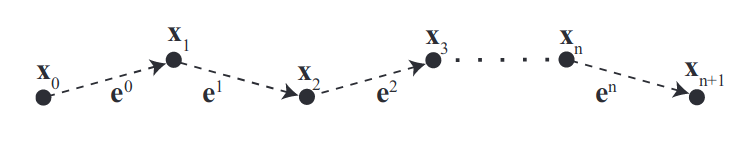
\includegraphics[width=0.85\textwidth]{img/discrete-edge.png}
	\caption{Centerline discretization}
\end{figure}

然后,我们为每一条\textbf{边}赋予一个材料标架 $\left\lbrace T^i, M_1^i, M_2^i \right\rbrace, i = 0, 1, \cdots, n$,其中 $T^i = \frac{e^i}{\left|e^i\right|}$  之所以对边而不是点赋予标架,是因为切向量天然地属于边,而将每一条边看作无形变的一小段圆柱也符合分段线性的思想。

此外,作为不可拉伸的离散形式,我们加上 constraint $\left|e^i\right| = \left|\overline{e}^{i}\right|$

\subsubsection{Discrete Bishop Frame}

除材料标架之外,我们还需要给折线段上的每个非顶点赋予一个 Bishop 标架,初始值 $\left\lbrace T^0, U^0, V^0 \right\rbrace$ 是任取的,在连续的情况下,其余的 Bishop 标架是通过求解微分方程得到的,现在我们就要将这个微分方程转换成\textbf{同等含义}的离散的递推公式(\textbf{而不是直接离散化,这样会出现数值误差})。

之前我们说过,之所以定义 Bishop Frame 作为参考,就是因为它没有 twist,\textbf{这是我们离散化时必须保持的性质}。同时,Bishop Frame 是 adapted frame,因此切向量确定。

由第一条性质,同一条边上的 Bishop 标架是常数 $\left\lbrace T^i, U^i, V^i \right\rbrace$。

而边与边之间的 Bishop 标架要满足无 twist 这个条件,则在顶点处旋转标架时的转轴必须垂直于 $T^i$ 和 $T^{i - 1}$。

两个条件合在一起,如果我们设在 $x_i$ 处标架的旋转矩阵为 $P_i$,则它应该满足关系式:

\begin{equation}
	\begin{aligned}
		&P_i(T^i \times T^{i - 1}) = T^i \times T^{i - 1} \\
		&P_i(T^{i - 1}) = T^i
	\end{aligned}
\end{equation}

由这个式子就可以解出 $P_i$,进一步可以由 $U^{i - 1}, V^{i - 1}$ 算出 $U^i, V^i$。递推即可得到所有点的 Bishop Frame

\begin{remark}
	请注意,在连续的情况下我们用 Darboux 向量来表示标架的旋转,然而这里却不能直接这么做,原因是 $T' \cdot T = 0$,但在离散的情况下,$T^{i}$ 未必垂直于 $T^{i - 1}$,所以不能指望 $\Omega \times T^{i - 1} = T^i$
\end{remark}

\begin{remark}
	实际写代码的时候这里不妨用四元数表示
\end{remark}

\subsubsection{Discrete Parallel Transport}

定义了 Bishop Frame 之后,平移就是显而易见的了。

在同一条边上,标架场保持不变,因此平移就是欧氏空间中的平移。

在顶点 $x_i$ 处,将向量从顶点的一侧平移到另一侧需要乘上旋转矩阵 $P_i$

\subsection{Discretization of Curvature and Darboux Vector}

\begin{definition}
	定义在顶点 $x^i$ 处的曲率为
	
	\begin{equation}\label{eq:discurvature}	
		k_i = 2 \tan (\frac{\phi_i}{2})
	\end{equation}

	其中 $\phi_i = <t^{i - 1}, t^i>$
\end{definition}

\begin{remark}
	我们并不关心这样定义的曲率的正负(实际上三维空间中的曲线的曲率在连续情况下按照定义都是正数),因为使用的时候都是用的是曲率的平方
\end{remark}

\begin{definition}
	定义在顶点 $x^i$ 处的 Darboux 向量为:

	\begin{equation}\label{eq:disdarboux}
		k_ib_i = \frac{2e^{i - 1} \times e^i}{\left|\bar{e}^{i - 1}\right|\left|\bar{e}^i\right| + e^{i - 1} \cdot e^i} 
	\end{equation}
\end{definition}

正如数学上的任意定义一样,这两个定义肯定也有背后的 motivation,我们之后再讲,在这里我们只需要注意到 $\left|k_ib_i\right| = \left|k_i\right|$ 以及 $t^{i} \rightarrow - t^{i - 1} \Rightarrow k_i \rightarrow \infty$,这两者是符合直观的。

\subsection{Discretization of Physics}

在定义了相关的几何量之后,物理量的计算也就是显而易见的了:

\begin{definition}
	离散化后的扭转势能为:

	\begin{equation}
		\begin{aligned}
			E_{twist}(\Gamma) &= \frac{1}{2} \beta\sum\limits_{i = 1}^{n} \left(\frac{\theta^{i} - \theta^{i - 1}}{\bar{l}_i / 2} \right)^2 \frac{\bar{l}_i}{2}  \\
			&= \beta \sum\limits_{i = 1}^{n} \frac{(\theta^i - \theta^{i - 1})^2}{\bar{l}_i}
		\end{aligned}
	\end{equation}
\end{definition}

\begin{remark}
	在这里我们是在边的中点上进行采样,用一阶差分来代替导数。
\end{remark}

\begin{definition}
	对于各项同性、rest shape 为直线的 rod,离散化后的弯曲势能为:

	\begin{equation}
		\begin{aligned}
			E_{bend}(\Gamma) &= \frac{1}{2} \alpha \sum\limits_{i = 1}^{n} \left(\frac{k_i}{\bar{l}_i / 2} \right)^2 \frac{\bar{l}_i}{2} \\
			&= \alpha \sum\limits_{i = 1}^{n} \frac{k_i^2}{\bar{l}_i} 
		\end{aligned}
	\end{equation}
\end{definition}

对于一般的 rod,离散化后的弯曲势能和 $\omega$ 有关,然而 $\omega$ 是 $T'$ 和 $M_1, M_2$ 的导数,可 $T'$ 是在顶点处定义的,而 $M$ 是在边上定义的,所以我们要拆成两半进行计算。首先注意到 $T' = kN$,但是我们只定义了 $kB$,我们需要用 $B$ 和 $M_1, M_2$ 的点积来表示 $\omega$:

\begin{figure}[H]
	\centering
	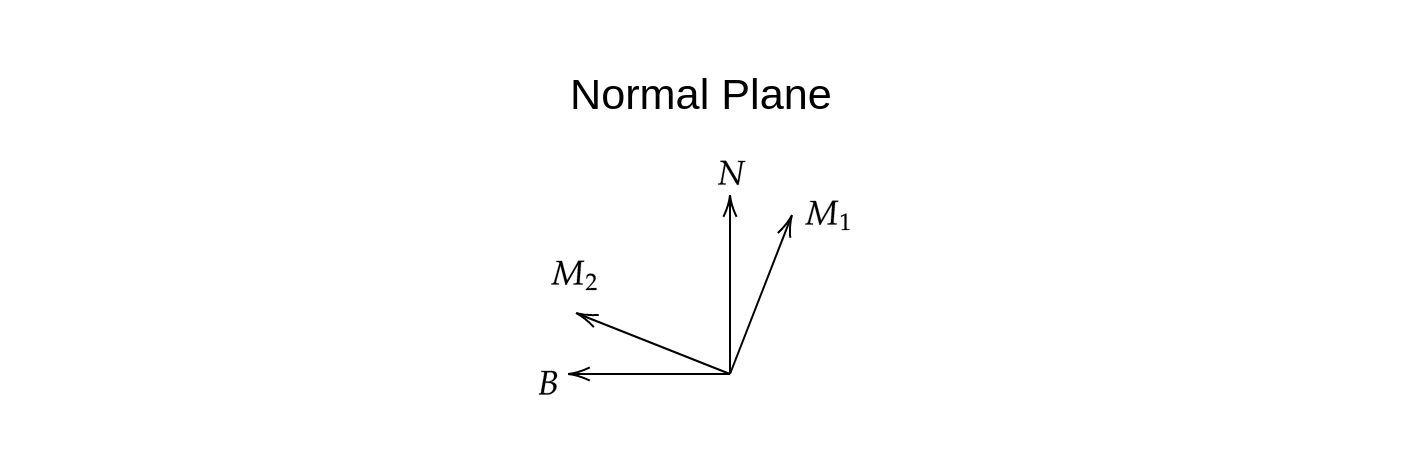
\includegraphics[width=0.85\textwidth]{img/normal-plane.png}
	\caption{Normal Plane}
\end{figure}

因此:

$$N \cdot M_1 = B \cdot M_2, N \cdot M_2 = -B \cdot M_1$$

即,若用 $\omega_i^j$ 表示第 $x_i$ 处的曲率信息和 $e^j(j = i - 1, i)$ 处的材料标架算出来的 $\omega$ 向量,则:

\begin{equation}
	\begin{aligned}
		\omega_i^j &= (k_iN_i \cdot M_1^j, k_iN_i \cdot M_2^j) \\
		&= (k_iB_i \cdot M_2^j, - k_iB_i \cdot M_1^j)
	\end{aligned}
\end{equation}

因此:

\begin{definition}
	对于一般的 rod,离散化后的弯曲势能为:

	\begin{equation}
		\begin{aligned}
			E_{bend}(\Gamma) &= \frac{1}{2} \sum\limits_{i = 1}^{n} \sum\limits_{j = i - 1, i}\left(\frac{\omega_i^j - \bar{\omega}_i^j}{\bar{l}_i / 2} \right)^T B \left(\frac{\omega_i^j - \bar{\omega}_i^j}{\bar{l}_i / 2} \right) \frac{\bar{l}_i}{4} \\
			&= \sum\limits_{i = 1}^{n} \frac{1}{2 \bar{l}_i} \sum\limits_{j = i - 1, i} (\omega_i^j - \bar{\omega}_i^j)^T B (\omega_i^j - \bar{\omega}_i^j)
		\end{aligned}
	\end{equation}
\end{definition}

\begin{remark}
	这里拆成两半算的时候原理上讲应该分别乘上 $\frac{\left|e^{i - 1}\right|}{2}$ 和 $\frac{\left|e^i\right|}{2}$,但这样的公式就太难看了……
\end{remark}

\subsection{Quasistatic Treatment of Material Frame}

我们目前只讨论 clamped end(stress free end 是显然的),公式 \ref{eq:minimize} 的离散形式是:

\begin{equation}\label{eq:disminimize}
	\frac{\partial E}{\partial \theta^i} = 0, i = 1, 2, \cdots, n - 1
\end{equation}

\begin{remark}
	但是值得注意的是,$\frac{\partial E}{\partial \theta^0}$ 和 $\frac{\partial E}{\partial \theta^n}$ 不一定是 $0$
\end{remark}

对于各项同性、rest shape 为直线的 rod,这等价于:

$$
	\begin{aligned}
	\frac{\partial E(\Gamma)}{\partial \theta^i} &= \frac{\partial }{\partial \theta^i} \sum\limits_{i = 1}^{n}\alpha k_i^2 / \bar{l}_i + \beta \frac{(\theta^i - \theta^{i - 1})^2}{\bar{l}_i} \\
	&= 2\beta\left(\frac{\theta^i - \theta^{i - 1}}{\bar{l}_i} - \frac{\theta^{i + 1} - \theta^i}{\bar{l}_{i + 1}}  \right) = 0
	\end{aligned}
$$

从而:

\begin{equation}
	\frac{\theta^i - \theta^{i - 1}}{\bar{l}_i} = \frac{\theta^{i + 1} - \theta^i}{\bar{l}_{i + 1}} = C, i = 1, 2, \cdots, n - 1
\end{equation}

从而:

$$\theta^n - \theta^0 = \sum\limits_{i = 1}^{n} \theta^i - \theta^{i - 1} = C \sum\limits_{i = 1}^{n} \bar{l}_i \Rightarrow C = \frac{\theta^n - \theta^0}{\sum\limits_{i = 1}^{n}\bar{l}_i}$$

设 $2 \overline{L} = \sum\limits_{i = 1}^{n} \bar{l}_i$(注意,$\bar{L}$ \textbf{不是} rod 的原长!),则我们可以把能量写成:

\begin{theorem}
	各项同性、rest shape 为直线的 rod 的扭转势能只与 $\theta$ 的差量有关,总能量为:
	\begin{equation}\label{eq:distwist}
		E(\Gamma) = \sum\limits_{i = 0}^{n}\alpha \frac{k_i^2}{\bar{l}_i} + \beta \frac{\left(\theta^n - \theta^0\right)^2}{2 \bar{L}}  
	\end{equation}
\end{theorem}

上述的推导过程中我们利用了 $k_i$ 与 $\theta$ 无关,因此 $E_{bend}$ 与 $\theta$ 无关,但对于一般的 rod,就没有这种好事了。因为 $\omega_i^j$ 和 $M^j_{1,2}$ 有关,而后者又和 $\theta^j$ 有关。

由 $\theta$ 的定义:

$$
	\left\{\begin{aligned}
		M_1^i &= \cos \theta^i U^i + \sin \theta^i V^i \\
		M_2^i &= - \sin \theta^i U^i + \cos \theta^i V^i
	\end{aligned}\right.
	\Rightarrow
	\left\{\begin{aligned}
		\frac{\partial M_1^i}{\partial \theta^i} &= - \sin \theta^i U^i + \cos \theta^i V^i = M_2^i\\
		\frac{\partial M_2^i}{\partial \theta^i} &= - \cos \theta^i U^i - \sin \theta^i V^i = - M_1^i
	\end{aligned}\right.
$$

进一步可以得到:

\begin{equation}
	\begin{aligned}
		\frac{\partial \omega_i^j}{\partial \theta^j} &= \frac{\partial }{\partial \theta^j} (k_iB_i \cdot M_2^j, -k_i B_i \cdot M_1^j) \\
		&= (-k_1B_i \cdot M_1^j, -k_iB_i \cdot M_2^j) \\
		&= J \omega_i^j
	\end{aligned}
\end{equation}

其中 $J = \begin{bmatrix}0 & 1 \\ -1 & 0\end{bmatrix}$

于是我们可以推导出:

\begin{equation}
	\begin{aligned}
		\frac{\partial E_{bend}(\Gamma)}{\partial \theta^i} &= \frac{\partial }{\partial \theta^i} \sum\limits_{i = 1}^{n} \frac{1}{2 \bar{l}_i} \sum\limits_{j = i - 1}^{i} (\omega_i^j - \bar{\omega}_i^j)^T B^i (\omega_i^j - \bar{\omega}_i^j) \\
		&= \sum\limits_{j = i, i + 1}\frac{1}{\bar{l}_{j}}(\omega_j^i - \bar{\omega}_j^i)^T(B^i)^T \frac{\partial \omega_j^i}{\partial \theta^i} \\
		&= \sum\limits_{j = i, i + 1} \frac{1}{\bar{l}_{j}}(\omega_j^i - \bar{\omega}_j^i)^T(B^i)^T J\omega_j^i
	\end{aligned}
\end{equation}

\begin{notation}
	为方便起见,记

	$$W^i_j = \frac{1}{2 \bar{l}_{j}}(\omega_j^i - \bar{\omega}_j^i)^T(B^i)^T (\omega_j^i - \bar{\omega}_j^i)$$

	以及

	$$m_i = \theta^{i} - \theta^{i - 1}$$

	则

	$$\frac{\partial W^i_j}{\partial \theta^j} = \frac{1}{\bar{l}_{j}}(\omega_j^i - \bar{\omega}_j^i)^T(B^i)^T J\omega_j^i$$
\end{notation}

再加上之前推出来的 $\frac{\partial E_{twist}(\Gamma)}{\partial \theta^i}$,我们得到:

\begin{equation}
	\frac{\partial E(\Gamma)}{\partial \theta^i} = \frac{\partial }{\partial \theta^i}(W_{i + 1}^i + W_{i}^i) + 2 \beta \left(\frac{m_i}{\bar{l}_i} - \frac{m_{i + 1}}{\bar{l}_{i + 1}}  \right) = 0
\end{equation}

这玩意是个非线性的方程,我们使用 Newton 迭代来求解,经过一通爆算,Hessian 为三对角矩阵:

\begin{equation}
	\begin{aligned}
		\frac{\partial ^2 E(\Gamma)}{\partial \theta^i \partial \theta^{i - 1}} &= - \frac{2 \beta}{\bar{l}_i} \\
		\frac{\partial ^2 E(\Gamma)}{\partial \theta^i \partial \theta^{i + 1}} &= - \frac{2 \beta}{\bar{l}_{i + 1}} \\
		\frac{\partial ^2 E(\Gamma)}{(\partial \theta^i)^2} &= \sum\limits_{j = i}^{i + 1} \frac{2 \beta}{\bar{l}_j} + \frac{1}{\bar{l}_j}(\omega_j^i)^TJ^T B^iJ \omega_j^i - \frac{1}{\bar{l}_j}(\omega_j^i - \bar{\omega}_j^i)^T B^i \omega_j^i 
	\end{aligned}
\end{equation}

\begin{remark}
	这里限于篇幅就没证明最后一个式子了,但最后一个式子的证明也不难,只要注意到 $J^2 = -I$ 和 $(B^i)^T = B^i$ 就好了
\end{remark}

\section{Dynamics of Elastic Rod}

经过对 $\theta$ 的 quasistatic 处理,rod 的自由度已经被减小到了所有的 $x_i$,现在的全部问题在于求绳子受的广义力:

$$-\nabla_{x_i} E(\Gamma)$$

\begin{remark}
	在做有限元的时候,我们经常需要求 Hessian,但这里不需要,因为作者懒了,直接用了个 semi-Euler
\end{remark}

但这里面最大的难点在于,$E(\Gamma)$ 是由 $\theta^i, x_i$ 共同描述的,因此我们必须要知道 $x_i$ 和 $\theta^i$ 的联系,即计算:

\begin{equation}
	\nabla_{x_i} E(\Gamma) = \frac{\partial E}{\partial x_i} + \sum\limits_{i = 0}^{n} \frac{\partial E}{\partial \theta^i} \frac{\partial \theta^i}{\partial x_i}
\end{equation}

幸运的是,对于 $i = 1, \cdots, n - 1$,由于 $\frac{\partial E}{\partial \theta^i} = 0$,后者都为 $0$。而 $\theta^0$ 取决于你的 Bishop 标架的选取,因此是任意的,我们可以固定为常数 $0$,所以上式化简为:

\begin{equation}
	\nabla_{x_i} E(\Gamma) = \frac{\partial E}{\partial x_i} + \frac{\partial E}{\partial \theta^n} \frac{\partial \theta^n}{\partial x_i}
\end{equation}

\begin{notation}
	下文为方便起见,记 $\nabla_i = \nabla_{x_i}$
\end{notation}

我们分别来求这三项:

首先,作为一切的核心,我们要求出 $(kB)_i$ 的导数,注意到 $(kB)_i$ 只和 $x_{i - 1}, x_i, x_{i + 1}$ 有关:

$$
	\begin{aligned}
	\nabla_{i - 1} (kB)_i &= \frac{\partial }{\partial x_{i - 1}} \frac{2 e^{i - 1} \times e^i}{\left|\bar{e}^{i - 1}\right| \left|\bar{e}^{i}\right| + e^{i - 1} \cdot e^i} \\
	&= \frac{\partial }{\partial x_{i - 1}} \frac{-2[e^i]e^{i - 1}}{\left|\bar{e}^{i - 1}\right| \left|\bar{e}^{i}\right| + e^{i - 1} \cdot e^i} \\
	&= \frac{2[e^i](\left|\bar{e}^{i - 1}\right| \left|\bar{e}^{i}\right| + e^{i - 1} \cdot e^i) + 2[e^i]e^{i - 1}(-e^i)^T}{(\left|\bar{e}^{i - 1}\right| \left|\bar{e}^{i}\right| + e^{i - 1} \cdot e^i)^2} \\
	&= \frac{2[e^i] + (kB)_i(e^i)^T}{\left|\bar{e}^{i - 1}\right| \left|\bar{e}^{i}\right| + e^{i - 1} \cdot e^i} 
	\end{aligned}
$$

类似的,我们得到:

\begin{equation}
	\begin{aligned}
		\nabla_{i - 1} (kB)_i &= \frac{2[e^i] + (kB)_i(e^i)^T}{\left|\bar{e}^{i - 1}\right| \left|\bar{e}^{i}\right| + e^{i - 1} \cdot e^i} \\
		\nabla_{i + 1} (kB)_i &= \frac{2[e^{i - 1}] - (kB)_i(e^{i - 1})^T}{\left|\bar{e}^{i - 1}\right| \left|\bar{e}^{i}\right| + e^{i - 1} \cdot e^i} \\
		\nabla_{i} (kB)_i &= -(\nabla_{i - 1} + \nabla_{i + 1}) (kB)_i
	\end{aligned}
\end{equation}

然后我们直接上一般情况下的导数:

% TODO

剩下的 $\frac{\partial \theta^n}{\partial x_i}$ 计算是最困难的,也是这篇文章最难懂的地方。

\subsection{The Impact of $x_i$ on $\theta$}

固定其他点,对 $x_i(0)$ 进行微小扰动,得到 $x_i(\varepsilon)$

\begin{figure}[H]
	\centering
	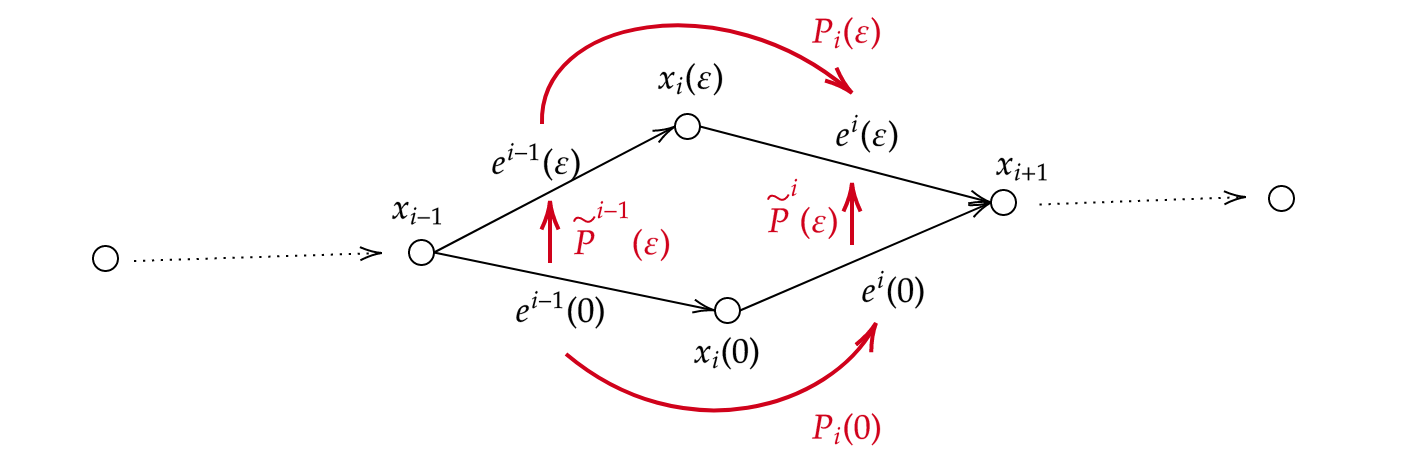
\includegraphics[width=0.85\textwidth]{img/holonomy.png}
	\caption{Variation of $x_i$}
\end{figure}

同一个向量,从 $x^{i - 1}$ 左侧的某一点出发,沿着 $x_i(\varepsilon)$ 所在的曲线,以之前定义的平移的方式移动到 $x_{i + 1}$ 右侧的一点所得到的向量,和沿着 $x_{i}(0)$ 所在的曲线平移得到的向量是一样的吗?

答案是否定的,用一两个例子就能够说明。而且,由于平移保证了切向量不变,且平移的所有过程中只涉及到向量的旋转,所以二者相差的将会是沿着切向量方向的转动 $\Delta \theta$ ,即导致 Bishop Frame 发生旋转,这正是我们想要捕捉的现象:$\theta^n$ 和 $x^i$ 相关联。

为了计算 $\Delta \theta$,注意到二者相差的是 $x_{i - 1} \rightarrow x_{i}(\varepsilon) \rightarrow x_{i + 1} \rightarrow x_i(0) \rightarrow x_{i - 1}$ 这个环路,因此,同一个向量沿着这个环路走一圈,得到的向量绕切向量旋转的角度就是二者相差的角度。

如图所示,在由平移 $P_i(0)$ 之外,我们额外定义了三个平移 $P_i(\varepsilon), \tilde{P}^{i - 1}(\varepsilon), \tilde{P}^{i}(\varepsilon)$,这三个平移的定义和 $P_i(0)$ 如出一辙,都是保证了切向量相互映射以及无 twist,即:

\begin{equation}
	\begin{aligned}
		&\tilde{P}^{j}(\varepsilon)t^j(0) = t^j(\varepsilon) \\
		&\tilde{P}^j(\varepsilon)(t^j(0) \times t^j(\varepsilon)) = t^j(0) \times t^j(\varepsilon)
	\end{aligned}
\end{equation}

\section{Putting it all together}

在有了之前的准备之后,我们的目标就只剩下了数值求解微分方程:

\begin{equation}
	M \ddot{x} = - \frac{d E(\Gamma)}{d x}
\end{equation}

其中 $x \in \mathbb{R}^{3(n + 2)}$ 而 $M \in \mathbb{R}{3(n + 2) \times 3(n + 2)}$ 为你分配给采样点的质量。

然而,之前说过,我们还要保证 $\left|e^i\right| = \left|\bar{e}^i\right|$ 这个 constraints。除此之外,我们还希望将 rod 的运动和 其他物体的运动藕合起来,比方说将 rod 的一头绑定在一个刚体上。为此,我们先叙述后者引起的 constraints,再说明如何处理 constraints。

\subsection{Rigid Body Coupling}

我们使用 $(q, r), q \in \mathbb{H}, r \in \mathbb{R}^3$ 表示一个刚体的运动,其中 $q$ 为单位四元数,表示物体的旋转,而 $r$ 表示物体的平移。如果我们的约束是将 rod 的第一节固定在刚体上,则对应的约束为:

\begin{equation}
	\begin{aligned}
		&q \cdot q = 1 \\
		&q \bar{x}_0 \bar{q} + r = x_0 \\
		&q \bar{x}_1 \bar{q} + r = x_1
	\end{aligned}
\end{equation}

其中第一项为单位四元数限制,第二项和第三项分别表示了根据刚体的运动和 rod 运动算出来的 rod 的第一节位置相同。

有很多种实现等式约束的方法,据我所知的最硬的方法是直接带 constraints 求解微分方程,即 Lagrange 乘子法,而最软的方法则是使用 penalty force。本文介绍的方法介于两者之间,它的目标是让单步迭代的结果落在 constraints manifold 上,但不追求微分方程的解的精确性。

\subsection{Fast Manifold Projection}

Fast Manifold Projection 的做法很简单:假设当前迭代在第 $n$ 步,广义坐标为 $y^n$,在无约束的情况下直接 step 一步,得到 $y^{n + 1}_0$ ,然后再 project 回到 constraint 上,即寻找

\begin{equation}\label{eq:optimization}
	y^{n + 1} = \min_{C(y^{n + 1}) = 0} d(y^{n + 1}_0, y^{n + 1})
\end{equation}


关键在于怎么定义度量 $d$,在这里我们使用离散化的动能

\begin{equation}
	d(x, y) = \frac{1}{2h^2} (x - y)^T M (x - y)
\end{equation}

我们使用拉格朗日乘子法求解优化问题 \ref{eq:optimization}。即求解:

\begin{equation}\label{eq:optimization2}
	(y^{n + 1}, \lambda) = \min_{\lambda, y^{n + 1}}\frac{1}{2h^2} \Delta y^T M \Delta y + C(y^{n + 1})^T \lambda
\end{equation}

其中 $\Delta y = y^{n + 1} - y^{n + 1}_0$

由于 $C$ 并非线性函数,优化问题 \ref{eq:optimization2} 只能通过迭代来求解,接下来我们忽略上标,设当前迭代数为 $k$,将 $C$ 在 $y_k$ 处展开得到:

$$C(y) \approx C(y_k) + \nabla C(y_k)(y - y_k)$$

对应的,第 $k$ 步我们求解二次优化问题:

\begin{equation}\label{eq:quadraticopt}
	(y_{k + 1}, \lambda_{k + 1}) = \min_{\lambda, y} \frac{1}{2h^2} (y - y_k)^T M (y - y_k) + (C(y_k) + \nabla C(y_k)(y - y_k))^T \lambda
\end{equation}

这个优化问题有解析解,直接对 $y, \lambda$ 求偏导就好了。

\begin{equation}
	\left\{\begin{aligned}
		&C(y_k) + \nabla C(y_k)(y - y_k) = 0 \\
		&\frac{1}{h^2} M(y - y_k) + \nabla C(y_k)^T \lambda = 0
	\end{aligned}\right.
	\Rightarrow
	\left\{\begin{aligned}
	&\lambda = \frac{1}{h^2} (\nabla C(y_k) M ^{-1} \nabla C(y_k)^T) ^{-1} C(y_k) \\
	&y_{k + 1} = y_k - h^2 M ^{-1} \nabla C(y_k)^T \lambda
	\end{aligned}\right.
\end{equation}

重复这个步骤直到收敛。最后,我们需要用 $y^{n + 1}$ 来重新计算速度,即 $v^{n + 1} = \frac{y^{n+1} - y^n}{h}$

\begin{remark}
	为什么不直接用 incremental potential 呢?我个人能够想到的唯一理由是 multibody system 中这样无约束求解这一步可以并行操作……但在 projective dynamic 里这个问题已经在某种意义上得到解决了……
\end{remark}

\subsection{General Coordinate of the Whole System}

最后,我们把整个系统中每个物理对象的广义坐标拼起来,得到整个系统的广义标架,在这里稍微提一嘴刚体的广义坐标 $(q, r)$,其角速度为向量 $2q ^{-1} \dot{q}$(这是一个纯四元数,我们将其看作是三维向量)。

整个系统的广义质量和对应的速度为(假设只有一个刚体,有多个刚体绑定 rod 的不同部位的话就把 rod 拆开来模拟)

\begin{equation}
	\tilde{M} = \begin{bmatrix}
		\mathcal{I} \\
		& M_{rigid} \cdot I_3 \\
		& &M_{rod}
	\end{bmatrix},
	v = \begin{bmatrix}
		2q ^{-1} \dot{q} \\
		\dot{r} \\
		\dot{x}
	\end{bmatrix}
\end{equation}



\end{document}
